\section{System implementation}
To compare performance of proposed AES circuit designs they were implemented in VHDL hardware description language and deployed on Terasic DE1-SoC development board. This chapter summarizes relevant to this research details of FPGA technology, describes implementation details of proposed AES designs and provides test results.
   
\subsection{Chosen hardware platform and development tools}
Terasic DE1-SoC development board \cite{plytka} was chosen to be a platform for deployment and testing of proposed designs. It is equipped with Altera Cyclone V SoC FPGA chip (5CSEMA5F31C6) \cite{cycloneVOverview}. This chip has (as reported by compilation report) 88277 logic elements and 32768 on-chip memory bits, which is enough for all of the tested designs.

All proposed designs were implemented in VHDL hardware description language. Quartus Prime Version 10.0.2 Lite Edition IDE was used to create, build and deploy the project. Simulation tests were conducted using ModelSim, which is a part of Quartus platform.

\subsection{Low level FPGA chip analysis}
\label{sec:low-level-fpga}
To optimize a circuit for high frequency operation it is necessary to understand how FPGA technology works on low level. FPGA chips' architectures may slightly vary, here focus is placed on architecture of the chip that was used for testing - Altera Cyclone V \cite[Chapter 1]{altera-vol1}. For simplicity only elements relevant to this research will be covered, detailed documentation is available in Cyclone V Handbook \cite{altera-vol1}.

FPGA chips consist of LABs (Logic Array Blocks), each of which contains 10 ALMs (Adaptive Logic Modules). ALMs are elements that make it possible to place arbitrary circuits in FPGA - they can be programmed to implement combinatorial logic functions, arithmetic functions, and registers.

Combinatorial logic is implemented in ALMS using LUTs (look-up tables) which contain high speed memory. This memory is programmed with precomputed outputs for every possible combination of logic levels of input signals. LUTs take combinatorial logic inputs and use them as addresses to corresponding memory bits. Output of LUT is a bit read from memory which corresponds to provided inputs. An important consequence of this design feature is that for a LUT with N inputs it is irrelevant how complex the logic to be implemented is - as long as it has no more than N inputs it will always perform the same. This is because all outputs are precomputed and all it takes to determine the output is to read it from memory. If desired combinatorial logic has more than N inputs multiple LUTs will be required.

In Cyclone V chips each ALM contains two LUTs and four registers (D flip-flops). The registers, however, are wired in such a way that only two are relevant for this design - other two could be utilised if ALMs were used to implement arithmetic logic, which does not happen in AES encryption. LUTs in Cyclone V ALMs are capable of implementing different combinations of combinatorial logic, for this design the relevant combinations are:
\begin{itemize}[noitemsep]
\item one 6-input LUT per ALM - uses up to 1 register, leaves at least one register unused
\item two 4-input LUTs per ALM - uses up to 2 registers
\end{itemize}

Combinatorial logic outputs can either be registered in the ALM they were calculated in or routed to another ALM without registering. For fastest operation in most cases it is desired to register them in the same ALM, because routing inside ALM is a lot faster than between ALMs. Routing outputs without registering is necessary when combinatorial logic has more inputs than a single ALM supports, or to move the register closer to other parts of the design to balance routing delays.

% Conducted tests showed that for AES encryption maximum frequency was higher for designs using only 4-input LUTs. Analysis of compilation reports showed that using 6-input LUTs resulted in overall increased number or resources used, which resulted in longer routing paths between parts of the design, which ultimately slowed it down. This makes sence, because for 4-input LUTs ALMs are used more efficiently - more combinatorial logic could be implemented, and both registers could be used. The leftover register when using 6-input operation mode was observed not to be used often, because other signals were typically registered in same ALMs they were calculated in.
Conducted tests showed that for AES encryption maximum frequency was higher for designs using only 4-input LUTs. Analysis of compilation reports showed that using 6-input LUTs resulted in paths with longer signal propagation time, which slowed the design down. This makes sense, because for 4-input LUTs ALMs are used more efficiently - more combinatorial logic could be implemented, and both registers could be used. The leftover register when using 6-input operation mode was observed not to be used often, because other signals were typically registered in same ALMs they were calculated in.

% Another important aspect of working with FPGA is that \textit{Place and Route} compilation phase, which is responsible of finding optimal placement of the design in FPGA chip, tackles an NP-hard problem. This phase therefore uses heuristics to produce an approximation of best possible solution. It is possible that final placement of the design will be different for each compilation attempt. This behaviour was observed during testing, but maximum frequency for given design remained stable between compilation attempts. The longest routes for each compilation were different every time, but leading trends were similar (eg. most routes from top 10 failing ones were between pipelined stages X and Y).


\subsection{VHDL description of the system's general structure}
All designed circuits have identical interfaces (fig. \ref{fig:top-aes}, lst. \ref{lst:entity}). As input they take:
\begin{itemize}[noitemsep]
\item \textbf{plaintext} -- 128b vector containing block of data to be encrypted
\item \textbf{key} -- 256b vector containing AES encryption key to be used
\item \textbf{clock} -- clock signal
\end{itemize}
All circuits output \textbf{cyphertext} -- 128b vector containing \textbf{plaintext} encrypted with \textbf{key}. Pipelined designs vary in number of \textbf{clock} cycles required for encryption process. Circuits do not input or output any control signals, it is up to the user of those entities to collect \textbf{cyphertext} after adequate number of \textbf{clock} cycles. Entity utilising \textit{Simple asynchronous architecture} does not use \textbf{clock} signal -- it is asynchronous.

\begin{figure}[!h]
\centering
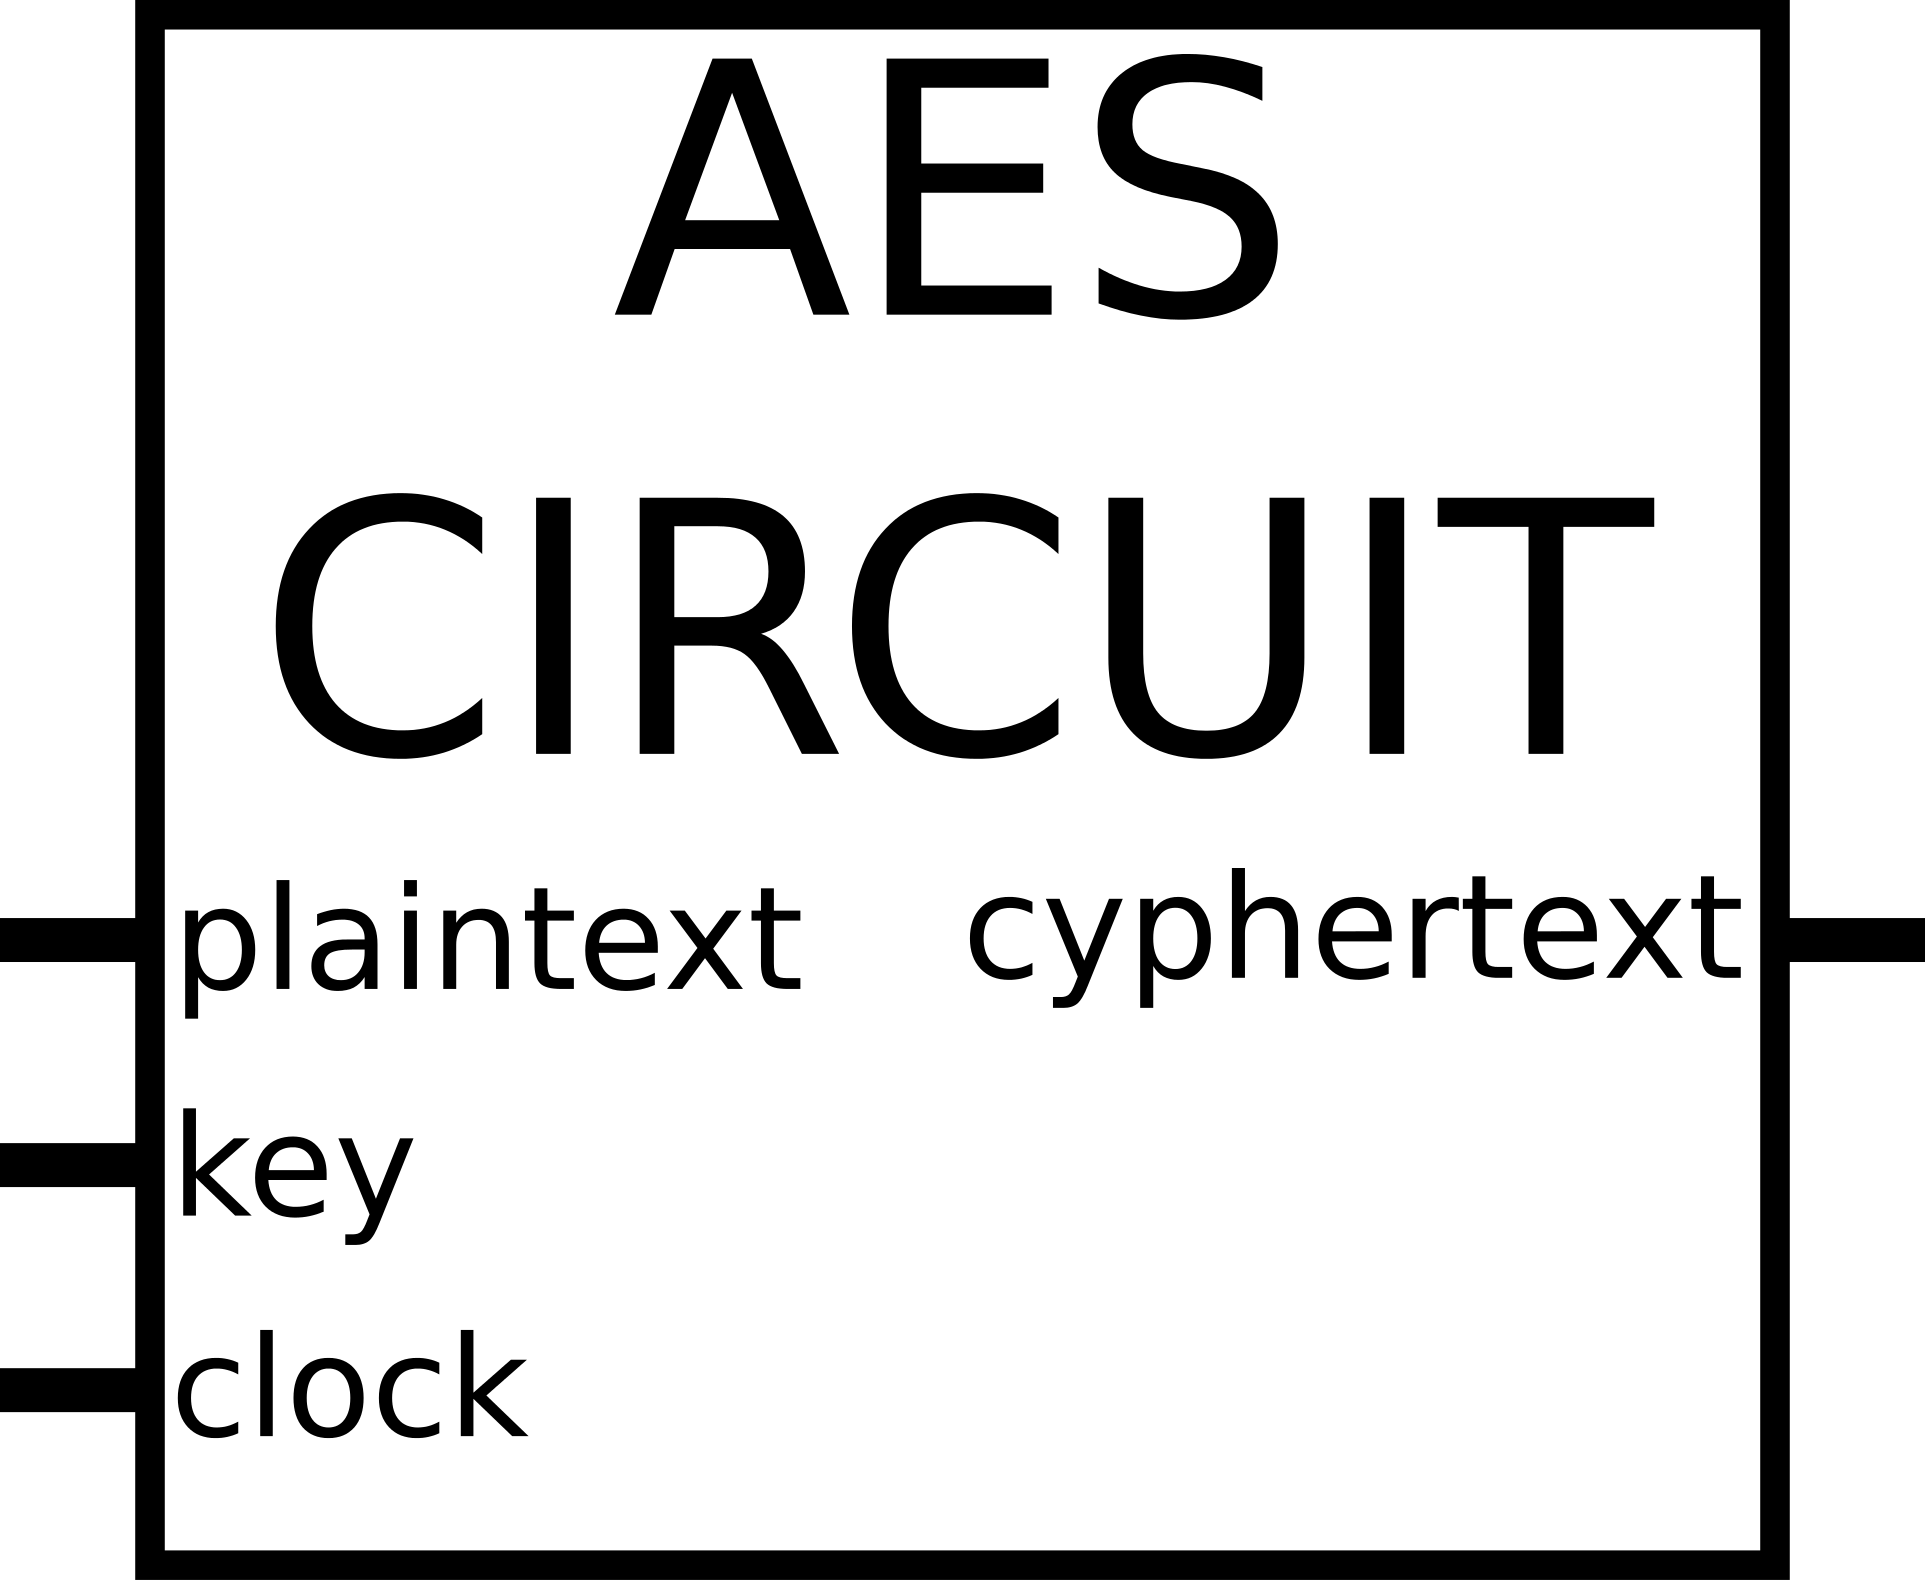
\includegraphics[scale=2]{top-aes}
\caption{Modified pipeline for pipelined rolled up architecture}
\label{fig:top-aes}
\end{figure}

\begin{figure}[!h]
\begin{lstlisting}[style=vhdl, caption={AES encryption VHDL entity}, label={lst:entity}, captionpos=b]
entity aes256enc is
	generic (
		block_bits    : Integer := 128);
	port (
		main_clk      : in  std_logic;
		key           : in  std_logic_vector(2 * block_bits - 1 downto 0);
		plaintext     : in  std_logic_vector(block_bits - 1 downto 0);
		cyphertext    : out std_logic_vector(block_bits - 1 downto 0)
	);
end aes256enc;
\end{lstlisting}
\end{figure}


\subsection{Implementation details of proposed designs}
This section provides implementation details of all designed AES encryption circuits.

\subsubsection{Simple asynchronous architecture}
Asynchronous AES encryption circuit is not clocked and does not implement any optimizations. Encryption is done at the speed of signal propagation. As Author showed in his BsC thesis \cite{inzynierka}, this design is capable of encrypting \textbf{20M blocks per second} (\textbf{2,5Gb/s} throughput). Compilation report shows that it uses \textbf{20797} (excluding 806 elements required for testing circuit - section \ref{sec:testing-methodology}) FPGA ALMs.

This design is described in detail in Author's past research - his BSc thesis \cite{inzynierka}.

\subsubsection{Pipelined unrolled architecture with stages of equal critical path length}

This design was implemented as part of this research as proposed in \cite{vlsi}.

Testing of the design showed that all transformations individually could run at frequencies exceeding 500MHz (close to or at testing circuits max frequency of 530MHz). One full round could run at this frequency as well, but adding more consecutive rounds resulted in decrease of frequency due to FPGA resource congestion resulting in longer routing paths. Full AES encryption circuit, which consists of 14 rounds, is capable of operating at \textbf{362MHz} and consumes \textbf{12564} ALM resources. Circuit operates with throughput of \textbf{46,3Gb/s} and encrypting a block of data requires \textbf{84} clock cycles.

Analysis of paths with longest propagation time presented in compilation report showed that typically they consisted of two or more ALMs used for calculating combinatorial logic. This was due to the fact that this design used pipelining stages which for calculating each output bit required more than 6 inputs. This forced utilising multiple ALMs between registers, which resulted in long routing delays.

The conclusions of this research were:
\begin{itemize}[noitemsep]
\item To achieve higher frequency it was necessary to split the design into shorter pipelining stages.
\item Critical path length calculated as number of layers of logical gates is irrelevant (sec. \ref{sec:low-level-fpga}).
\item What is relevant is the number of input signals required for calculating each bit of stage output, which should be no higher than 6.
\item Routing delays are a significant factor contributing to maximum achievable frequency.
\item Reducing number of LUTs between registers is critical for high performance.
\end{itemize}

\subsubsection{Pipelined unrolled architecture with stages containing one ALM}
\label{sec:implementation-pipe-unrolled-one-alm}

First approach to implementing this circuit was to split pipelining stages so that they used 4-input as well as 6-input LUTs. This approach resulted in increased performance, but analysis of compilation reports showed that paths with longest signal propagation time typically led through ALMs utilising 6-input operation mode. The circuit was therefore further redesigned to take advantage of only 4-input operation mode. Final design is capable of operating at \textbf{401MHz}, which is the highest achieved frequency for AES encryption observed in this research. The number of logic elements as reported by compiler for this design is \textbf{18078} (excluding 806 elements required for testing circuit). Circuit operates with throughput of \textbf{51,3Gb/s} and encrypting a block of data requires \textbf{154} clock cycles.

This section describes in detail how each operation in AES algorithm can be split into stages taking advantage of only 4-input LUT operation mode. To utilise this mode each registered output bit needs to depend on no more than 4 inputs.

\paragraph{Mapping $f(x)$ from $GF(2^8)$ to $GF((2^4)^2)$}\mbox{}\\
Output bits of this operation depend on as much as 7 input bits, therefore to make it use only 4-input LUTs it is necessary to split it into two substages (\ref{eg:f-split}) (fig. \ref{fig:f-split}) -- $f_a$ (\ref{eq:mul_delta_a}) and $f_b$ (\ref{eq:mul_delta_b}).

\begin{equation}
\label{eg:f-split}
f(x) = f_b \circ f_a(x)
\end{equation}

\begin{figure}[!h]
\centering
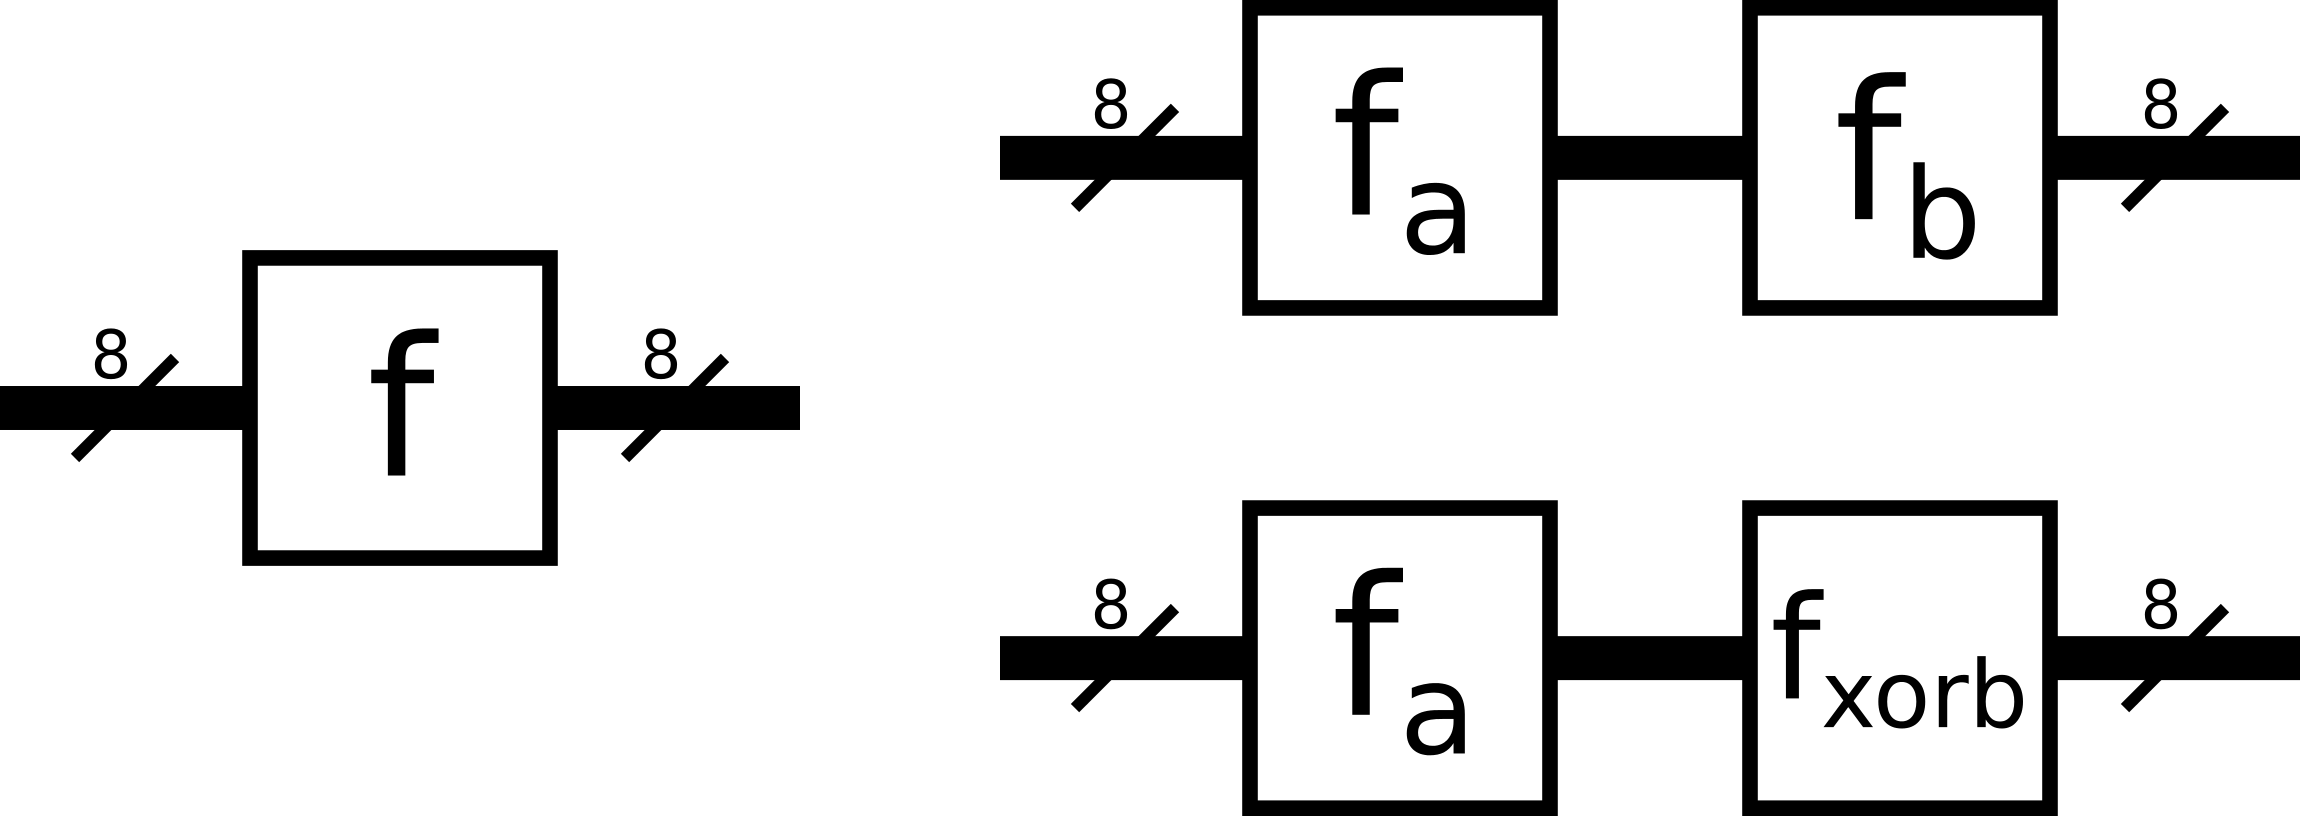
\includegraphics[scale=4]{f-split}
\caption{Decomposition of mapping $f(x)$ from $GF(2^8)$ to $GF((2^4)^2)$ into two stages}
\label{fig:f-split}
\end{figure}

\begin{figure}[!h]
\begin{multicols}{2}

\begin{equation}
\label{eq:mul_delta_a}
\begin{aligned}
b_{a0}    &= b_0                    \\
b_{a1}    &= b_1                    \\
b_{a2}    &= b_2                    \\
b_{a3}    &= b_3                    \\
b_{a4}    &= b_4                    \\
b_{a5}    &= b_5                    \\
b_{a6}    &= b_6                    \\
b_{a7}    &= b_7                    \\
b_{a23}   &= b_2 + b_3              \\
b_{a57}   &= b_5 + b_7              \\
b_{a14}   &= b_1 + b_4                
\end{aligned}
\end{equation}

\break
 
\begin{equation}
\label{eq:mul_delta_b}
\begin{aligned}
b'_0 &= b_{a0} + b_{a1} + b_{a6}           \\
b'_1 &= b_{a6} + b_{a14}                   \\
b'_2 &= b_{a7} + b_{a14} + b_{23}          \\
b'_3 &= b_{a1} + b_{a2} + b_{a6} + b_{a7}  \\
b'_4 &= b_{a1} + b_{a57} + b_{a23}         \\
b'_5 &= b_{a57} + b_{a23}                  \\
b'_6 &= b_{a6} + b_{a7} + b_{a14} + b_{a23}\\
b'_7 &= b_{a57}                            
\end{aligned}
\end{equation}

\end{multicols}
\end{figure}

\newpage
In SubBytes transformation after mapping $f(x)$ from $GF(2^8)$ to $GF((2^4)^2)$ high and low words of the result are xored together (fig. \ref{fig:mul_inv_gf242}). This operation can be performed concurently with $f_b(x)$ mapping to avoid creating a separate stage only for a xor operation.

\begin{equation}
\begin{aligned}
f_{xor}(x) &= f(x)_{low} + f(x)_{high} \\
f_{xor}(x) &= f_{xorb} \circ f_a(x)
\end{aligned}
\end{equation}

\begin{equation}
\label{eq:mul_delta_xor}
\begin{aligned}
b_{xorb0} &= b_{a0} + b_{a23} + b_{a567}       \\
b_{xorb1} &= b_{a1234} + b_{567}               \\
b_{xorb2} &= b_{a6}                            \\
b_{xorb3} &= b_{a1} + b_{a2} + b_{a5} + b_{a6}
\end{aligned}
\end{equation}

From equations (\ref{eq:mul_delta_a}), (\ref{eq:mul_delta_b}) and (\ref{eq:mul_delta_xor}) it is apparent that each stage output bit depends on no more than 4 inputs.




\paragraph{Mapping $f^{-1}(x)$ from $GF((2^4)^2)$ to $GF(2^8)$ combined with AES affine transformation}\mbox{}\\
Analoguously to mapping $f(x)$ from $GF(2^8)$ to $GF((2^4)^2)$, mapping $f^{-1}(x)$ from $GF((2^4)^2)$ to $GF(2^8)$ combined with affine transformation (\ref{sec:comb-theory}) (\ref{eq:fa-split}) (fig. \ref{fig:fa-split}) should be split into two substages --  $f^{-1}_a$ (\ref{eq:mul_delta_inf_a}) and $f^{-1}_b$ (\ref{eq:mul_delta_inf_b}).

\begin{equation}
\label{eq:fa-split}
\begin{aligned}
f^{-1}(x) &= f_b^{-1}(x) \circ f_a^{-1}(x) \\
\end{aligned}
\end{equation}

\begin{figure}[!h]
\centering
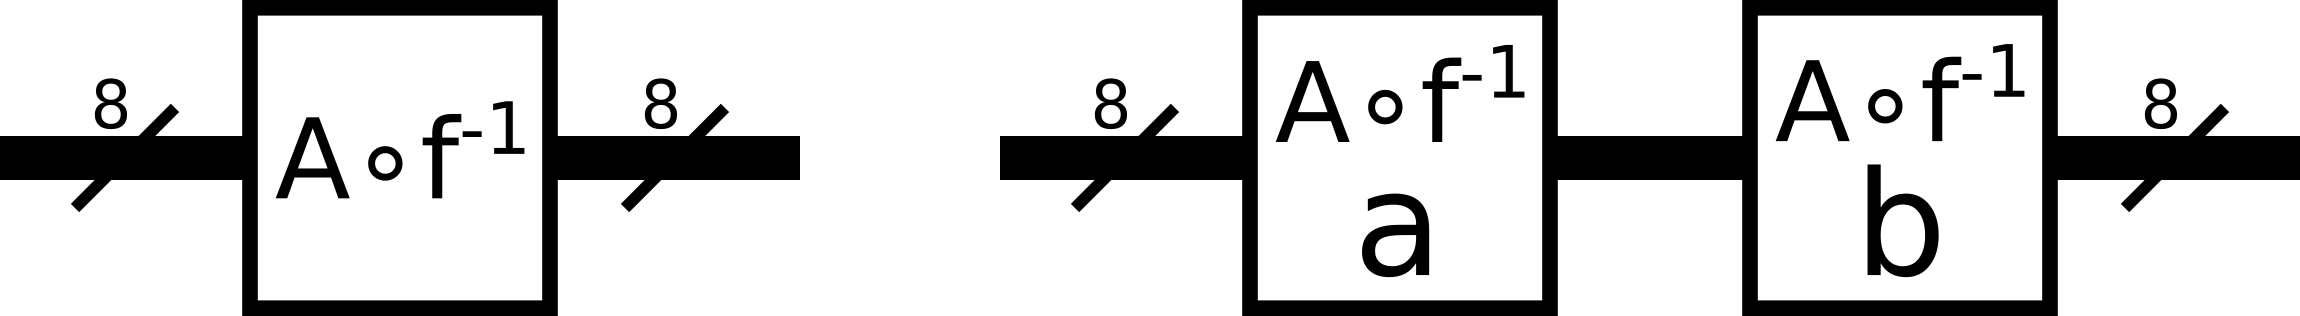
\includegraphics[scale=4]{fa-split}
\caption{Decomposition of mapping $f^{-1}(x)$ from $GF((2^4)^2)$ to $GF(2^8)$ combined with AES affine transformation into two stages}
\label{fig:fa-split}
\end{figure}


\begin{figure}[!h]
\begin{multicols}{2}

\begin{equation}
\label{eq:mul_delta_inf_a}
\begin{aligned}
b_{a0}    &= b_0                    \\
b_{a7}    &= b_7                    \\
b_{a23}   &= b_2 + b_3              \\
b_{a012}  &= b_0 + b_1 + b_2        \\
b_{a023}  &= b_0 + b_2 + b_3        \\
b_{a456}  &= b_4 + b_5 + b_6        \\
b_{a0147} &= b_0 + b_1 + b_4 + b_7  \\
b_{a27N}  &= b_2 + b_7 + 1          \\
b_{a67N}  &= b_6 + b_7 + 1            
\end{aligned}
\end{equation}

\begin{equation}
\label{eq:mul_delta_inf_b}
\begin{aligned}
b'_0 &= b_{a012} + b_{67N}           \\
b'_1 &= b_{a0} + b_{a7} + 1          \\
b'_2 &= b_{a023} + b_{a456}          \\
b'_3 &= b_{a012}                     \\
b'_4 &= b_{a0147}                    \\
b'_5 &= b_{a27N}                     \\
b'_6 &= b_{a456} + b_{a7} + 1        \\
b'_7 &= b_{a23} + b_{a7}                    
\end{aligned}
\end{equation}

\end{multicols}
\end{figure}

From equations (\ref{eq:mul_delta_inf_a}) and (\ref{eq:mul_delta_inf_b}) it is apparent that each stage output bit depends on no more than 4 inputs. Note that $xor$ with $1$ value is merely a $not$ operation, and it does not increase input count. It is also true that all outputs of $f_b^{-1}(x)$ stage depend on no more than 2 inputs, so they can be xored with 2 other independent inputs to form a stage, which is important for a stage in key expansion pipeline.




\paragraph{Multiplicative inversion in $GF(2^4)$}\mbox{}\\
This operation has only 4 inputs, so it is can already be implemented using a 4-input LUT.

\paragraph{Multiplication by constant $\phi$ in $GF(2^2)$}\mbox{}\\
This operation has only 2 inputs, so it is can already be implemented using a 4-input LUT. 

\paragraph{Multiplication by constant $\lambda$ in $GF(2^4)$}\mbox{}\\
This operation has only 4 inputs, so it is can already be implemented using a 4-input LUT. Moreover, it is only used as part of SubBytes transformation directly after squaring in $GF(2^4)$. Because squaring takes only 4 inputs, and multiplication by $\lambda$ operates only on output of squaring, those two operations can be combined into single stage. Such merging only increases length of critical path of the stage (which is irrelevant) but does not increase number of inputs, which is still 4.


\paragraph{Multiplication in $GF(2^2)$}\mbox{}\\
This operation has only 4 inputs, so it is can already be implemented using a 4-input LUT. Every output depends on at most 3 inputs, so it is possible to xor each of them with a signal that does not depend on anything (was just registered).

\paragraph{Multiplication in $GF(2^4)$}\mbox{}\\
This operation has 8 inputs, so it is necessary to split it into two stages (fig. \ref{fig:mul-gf4-split}).

\begin{figure}[!h]
\centering
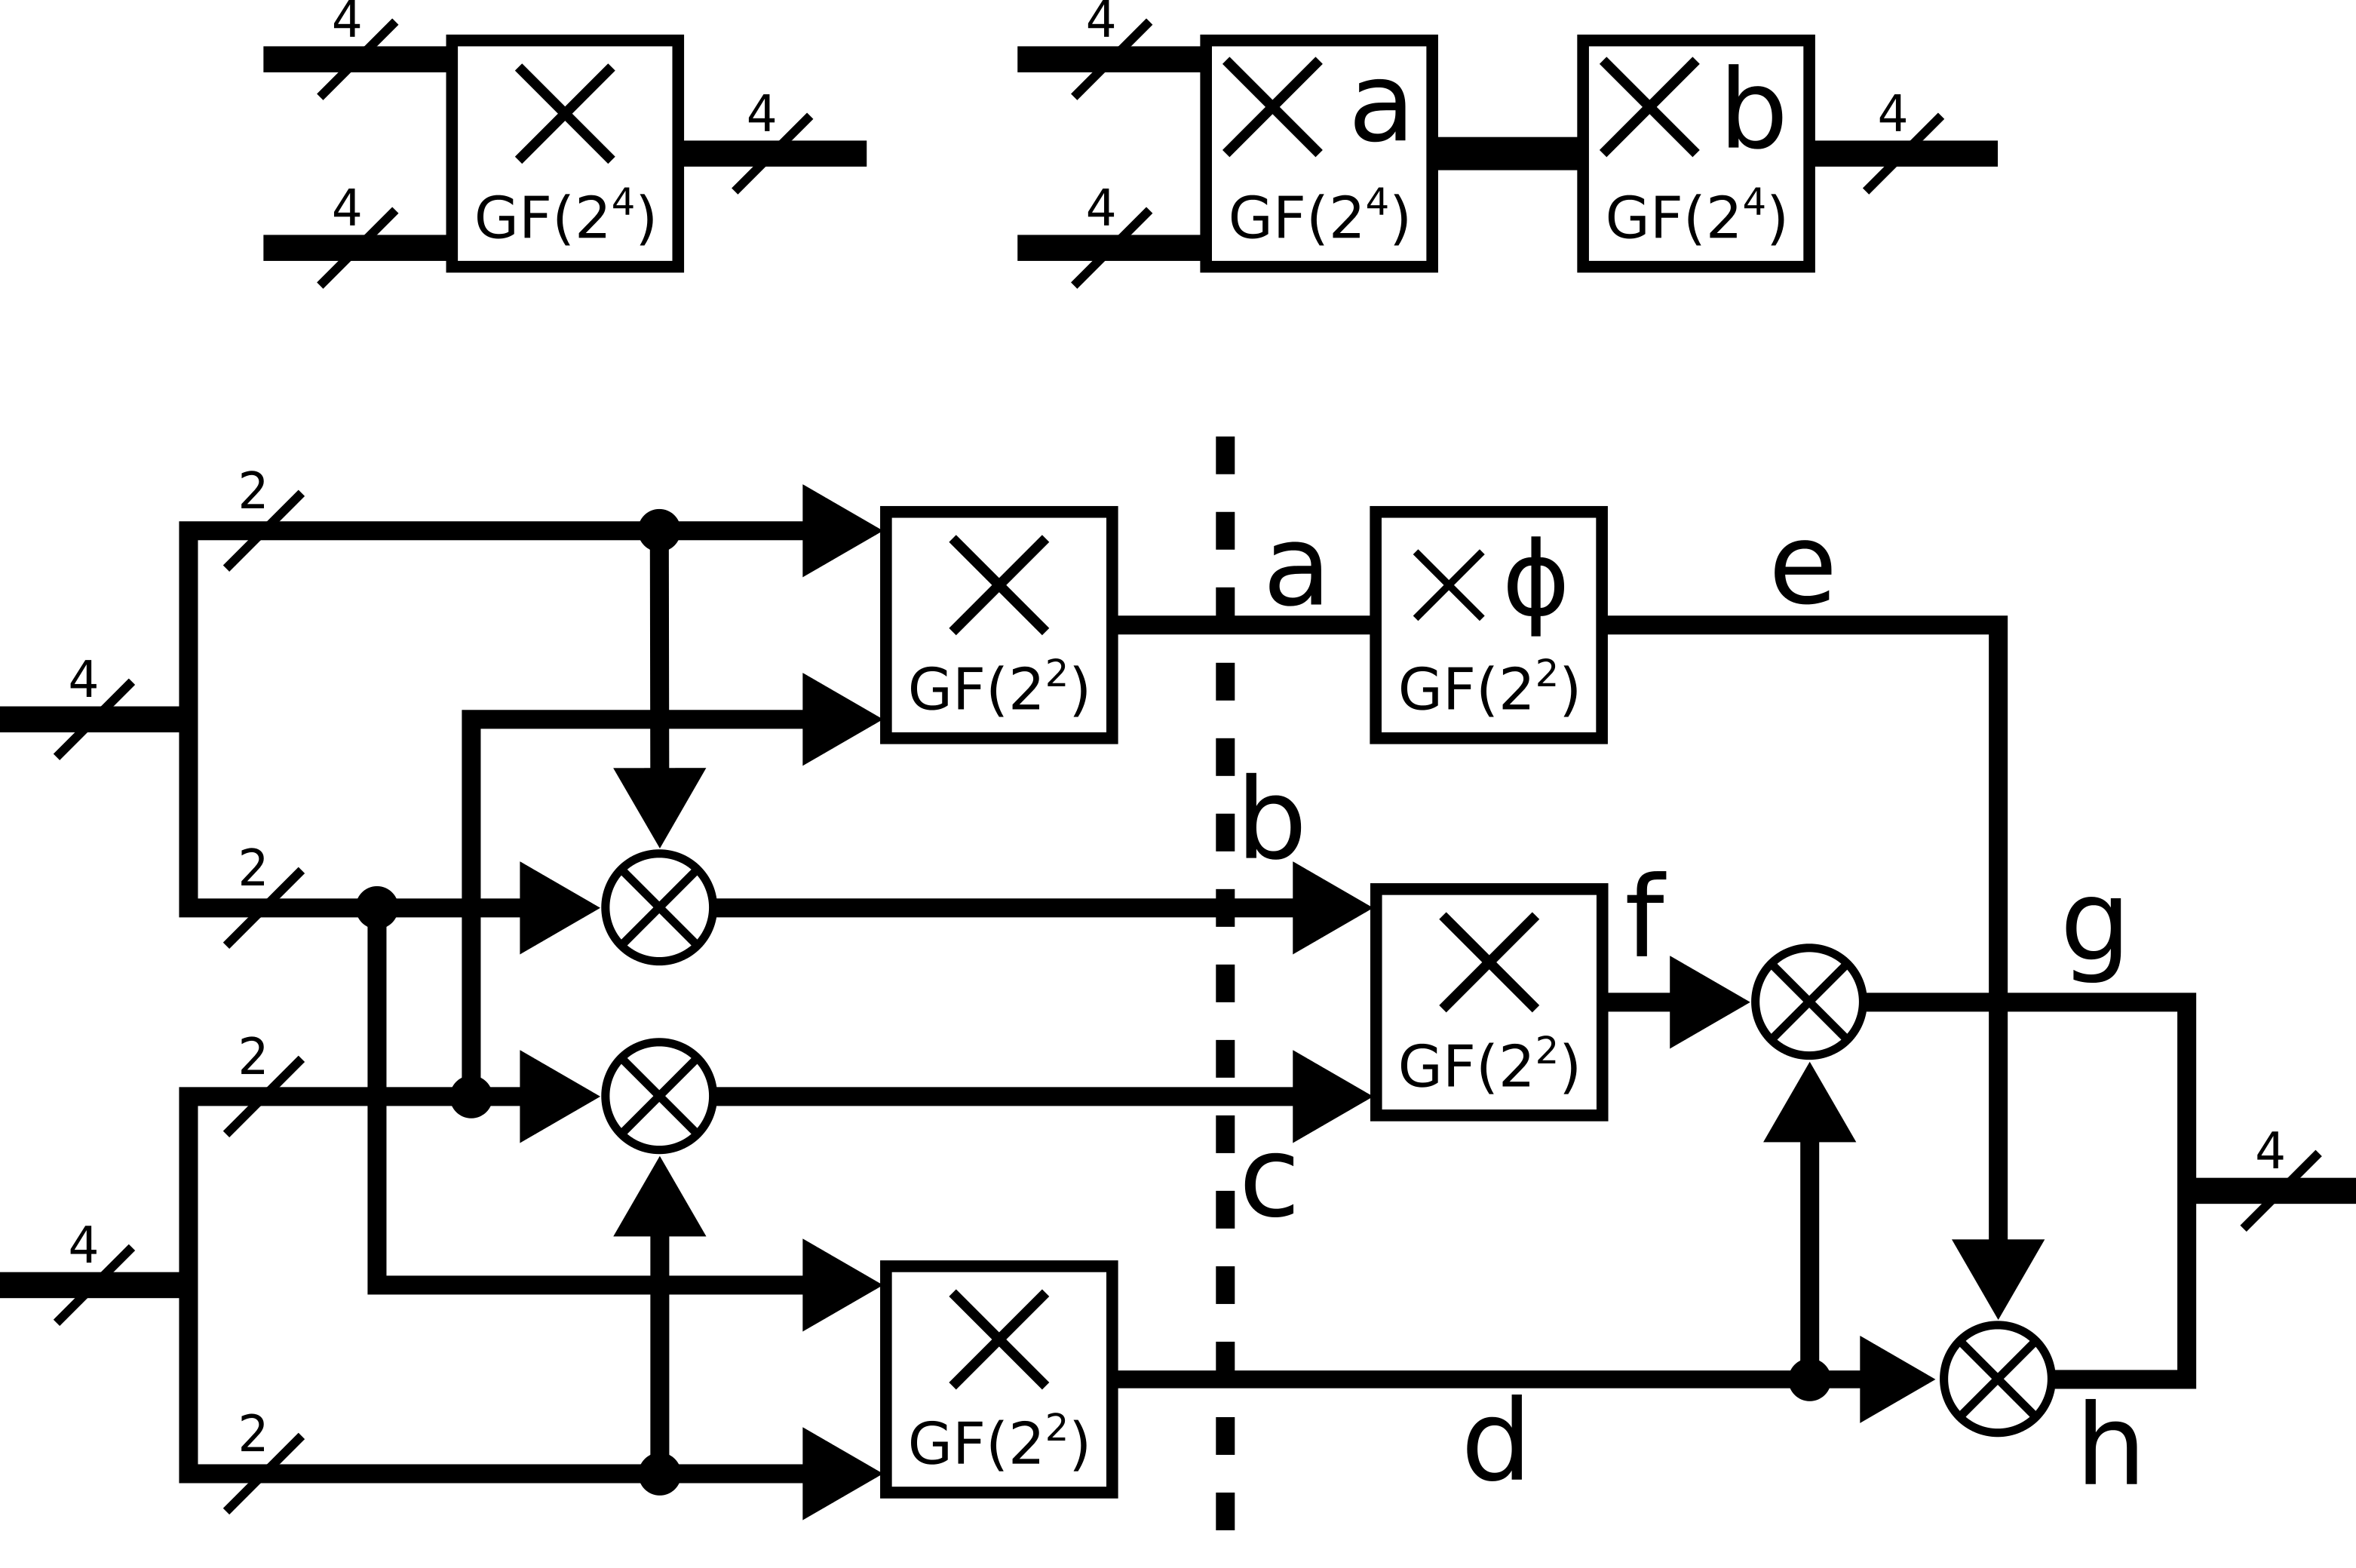
\includegraphics[scale=4]{mul-gf4-split}
\caption{Decomposition of multiplication in $GF(2^4)$ into two stages}
\label{fig:mul-gf4-split}
\end{figure}

This split uses only 4-input LUT operation mode, because:
\begin{itemize}[nolistsep]
\item Each bit of signals $a$ and $d$ depends on no more than 3 input signals, because on their paths there are only multiplications in $GF(2^2)$, which have this property. 
\item Each bit of signals $b$ and $c$ depends only on 2 input signals, because they are xors.
\item Each bit of signal $e$ depends on no more than 2 input signals, because this is a property of multiplication by $\phi$.
\item Each bit of signal $f$ depends on no more than 3 input signals, because this is a property of multiplication in $GF(2^2)$.
\item Each bit of signal $g$ depends on no more than 4 input signals, because signals from $f$ are xored with independent signals.
\item Each bit of signal $h$ depends on no more than 3 input signals, because signals from $e$ are xored with independent signals.
\end{itemize}


\paragraph{Squaring in $GF(2^4)$}\mbox{}\\
This operation has only 4 inputs, so it is can already be implemented using a 4-input LUT.


\paragraph{ShiftRows transformation}\mbox{}\\
This transformation does not do combinatorial logic and thus can be joined with any other operation to form a stage.


\paragraph{MixColumns transformation}\mbox{}\\
Lets first notice that some output bits of multiplication by $\{02\}_{16}$ depend on 2 input signals (\ref{eq:mul2}). In MixColumns transformation this multiplication is performed on signals which were are already $xored$ (fig. \ref{fig:mix_columns}). This means that outputs of multiplication by $\{02\}_{16}$ blocks already depend on $2 * 2 = 4$ signals. Those outputs are then xored again, which results in exceeding 4-input limit. MixColumns transformation, therefore, needs to be split into two stages. It can be done as shown in figure \ref{fig:mix-columns-split}.

\begin{figure}[!h]
\centering
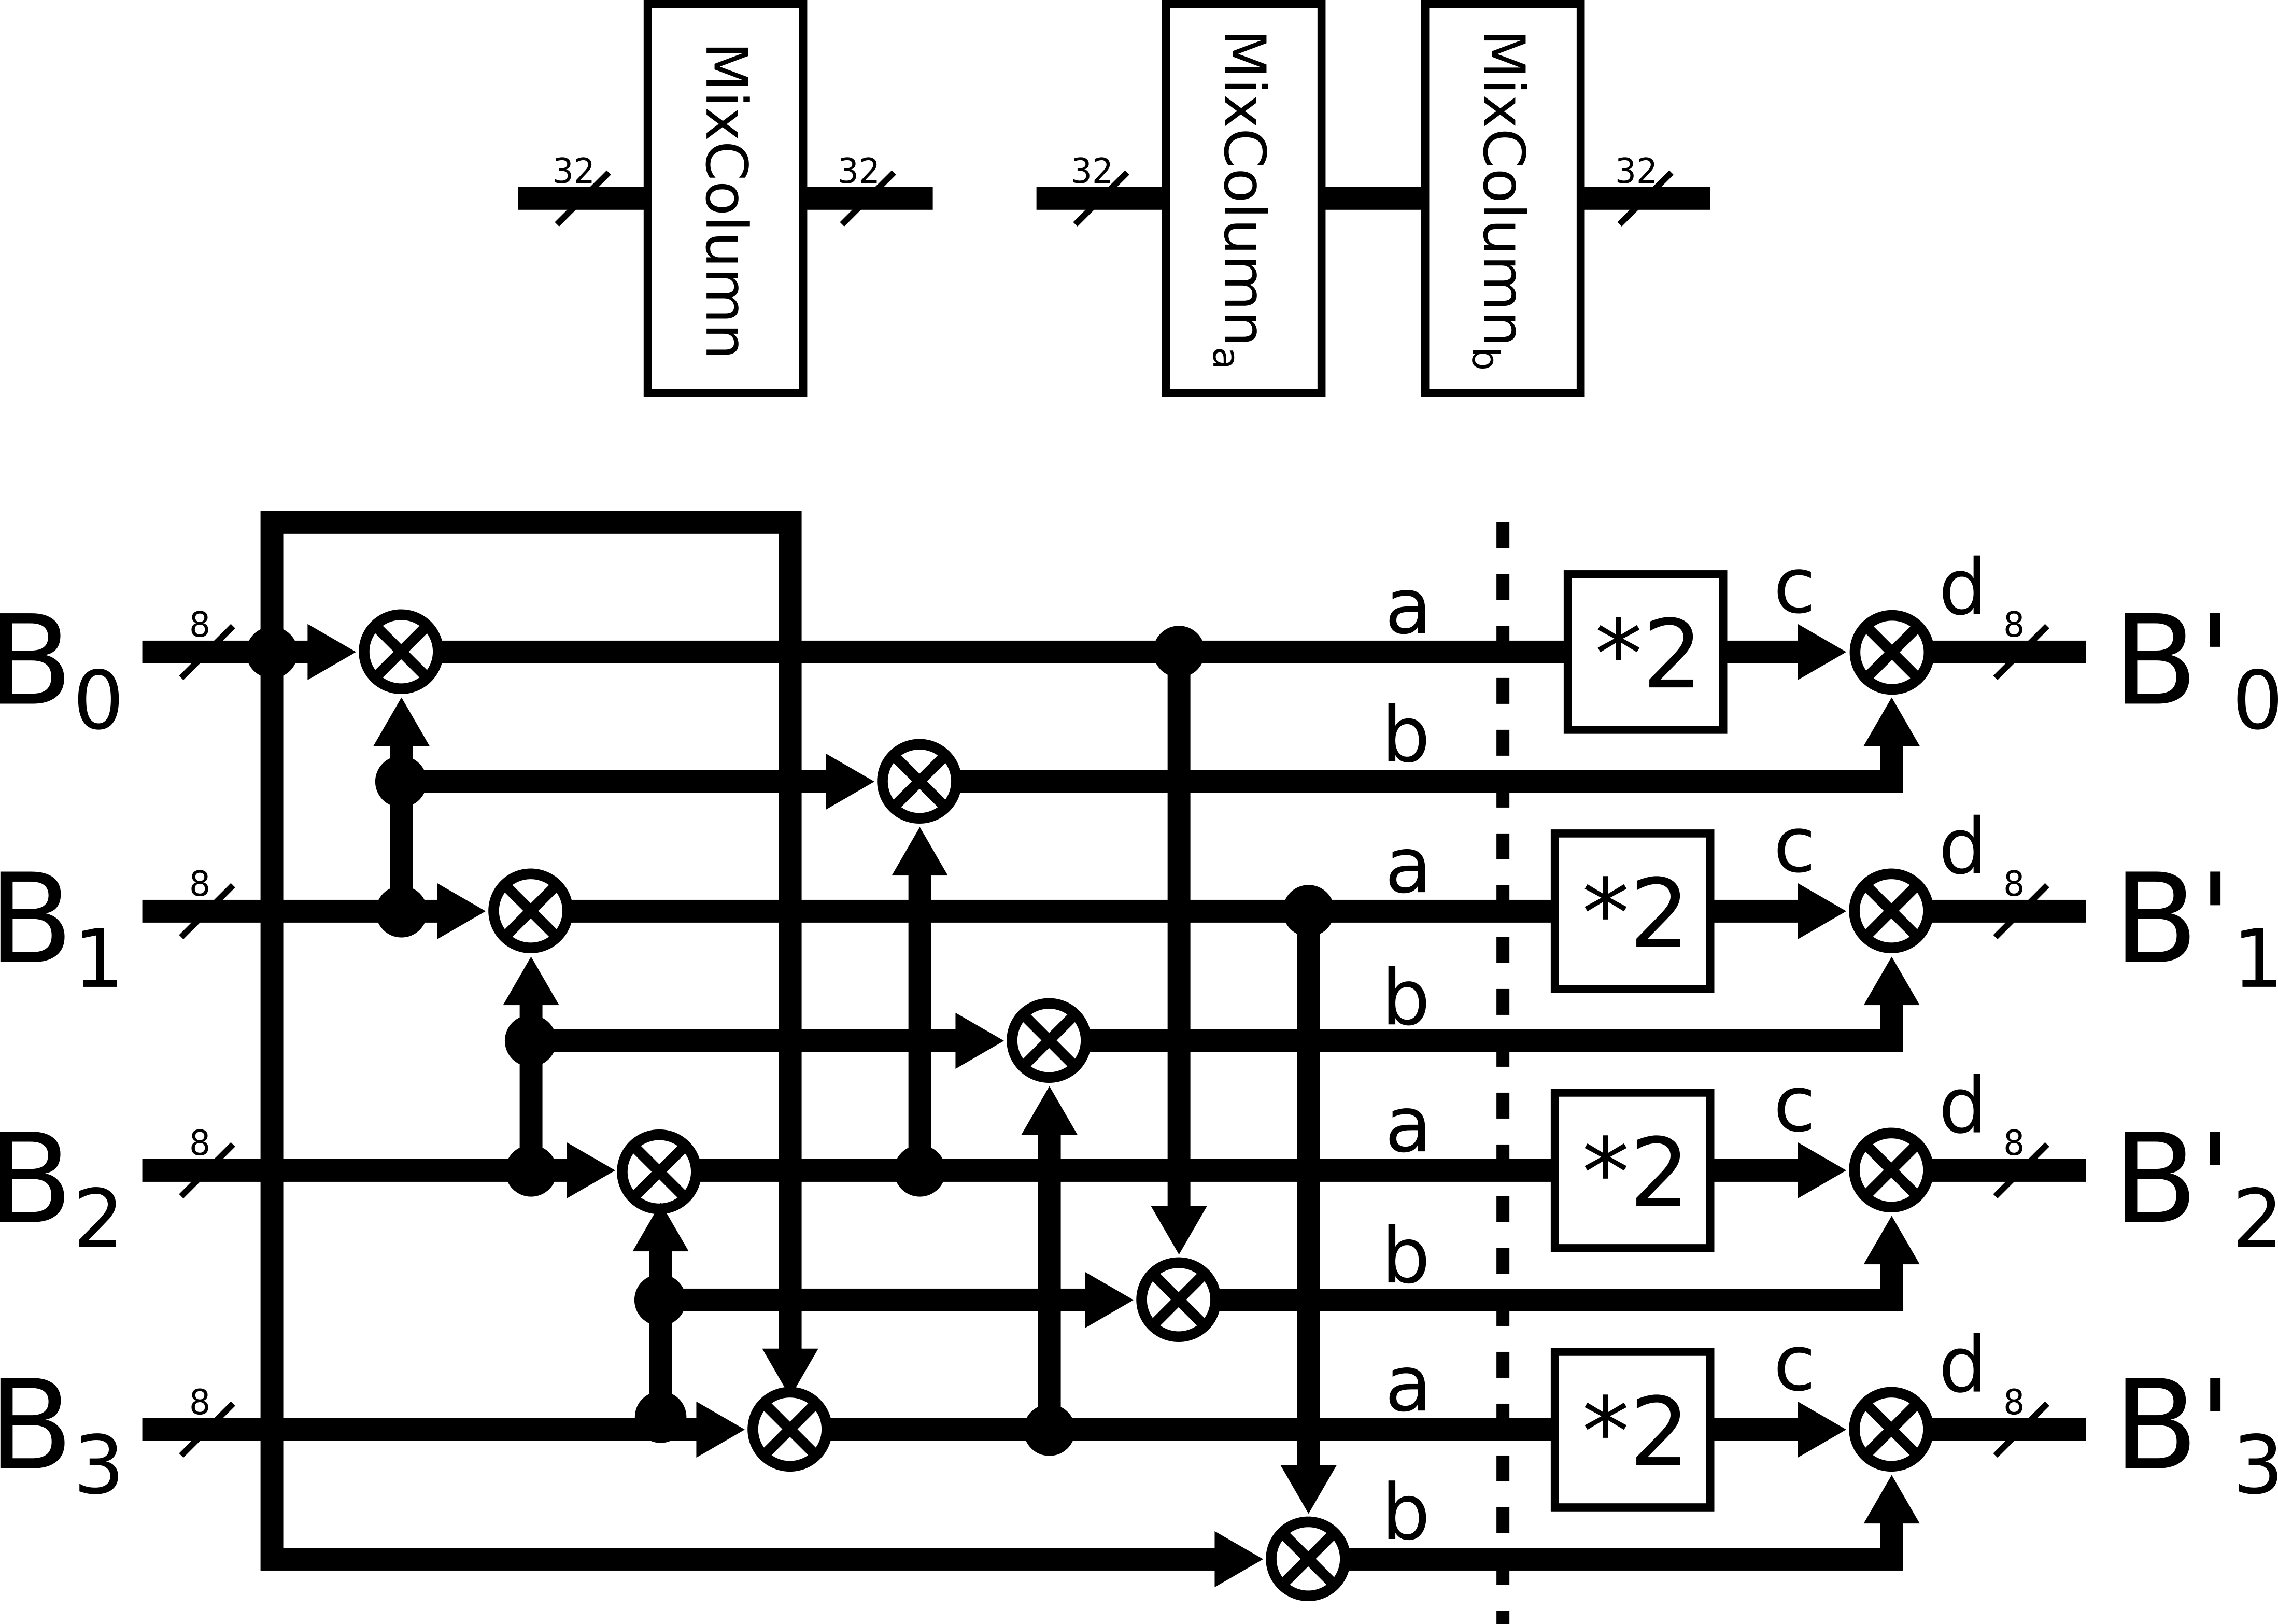
\includegraphics[scale=3]{mix-columns-split}
\caption{Decomposition of MixColumns transformation into two stages}
\label{fig:mix-columns-split}
\end{figure}

Those stages can be implemented using only 4-input LUTs, because:
\begin{itemize}[nolistsep]
\item Each bit of signals marked $a$ depends on 2 input signals.
\item Each bit of signals marked $b$ depends on 3 input signals.
\item Each bit of signals marked $c$ depends on no nore than 2 input signals.
\item Each bit of signals marked $d$ depends on no nore than 3 input signals.
\end{itemize}

Note that all output bits depend on no more than 3 input signals, which means that they can be $xored$ with other independent inputs in one stage. This is useful for combining it with AddRoundKey transformation.


\paragraph{AddRoundKey transformation}\mbox{}\\
This transformation consists only of a xor gate, which means that it can be combined into one stage with MixColumns.


\paragraph{$Rot$ operaiton in KeyExpansion}\mbox{}\\
$Rot$ operation rotates a word (4 bytes) left by one byte, therefore it does not require any combinatorial logic. Similarly to ShiftRows transformation it can be joined with any other operation to form a stage.

\paragraph{$Rcon$ operation in KeyExpansion}\mbox{}\\
$Rcon$ operation xors highest byte of a word with $2^{N + 1}$, which means that it adds at most one signal to input. It is performed after second stage of mapping $f^{-1}(x)$ from $GF((2^4)^2)$ to $GF(2^8)$ combined with AES affine transformation ($f_b^{-1}(x)$), outputs of which depend on only 2 input bits. This means that combining $f_b^{-1}(x)$ with $Rcon$ in a stage results in outputs depending on 3 bits, which still leaves space in this stage. This one extra signal is utilised in KeyExpansion pipeline.

\paragraph{Final design of throughput-optimized AES encryption circuit}\mbox{}\\
Taking all points presented in this section into consideration, it follows that a pipelied circuit using only 4-input LUTs can be implemeted according to diagram in figure \ref{fig:high-speed-pipe-full}.





\newpage


\subsubsection{Pipelined rolled up architecture with stages containing one ALM}

This design aims to reduce FPGA resource usage at the cost of reducing throughput by utilising rolling up of the pipeline (creating a loop) (fig. \ref{fig:rolled-loop}).

\begin{figure}[!h]
\centering
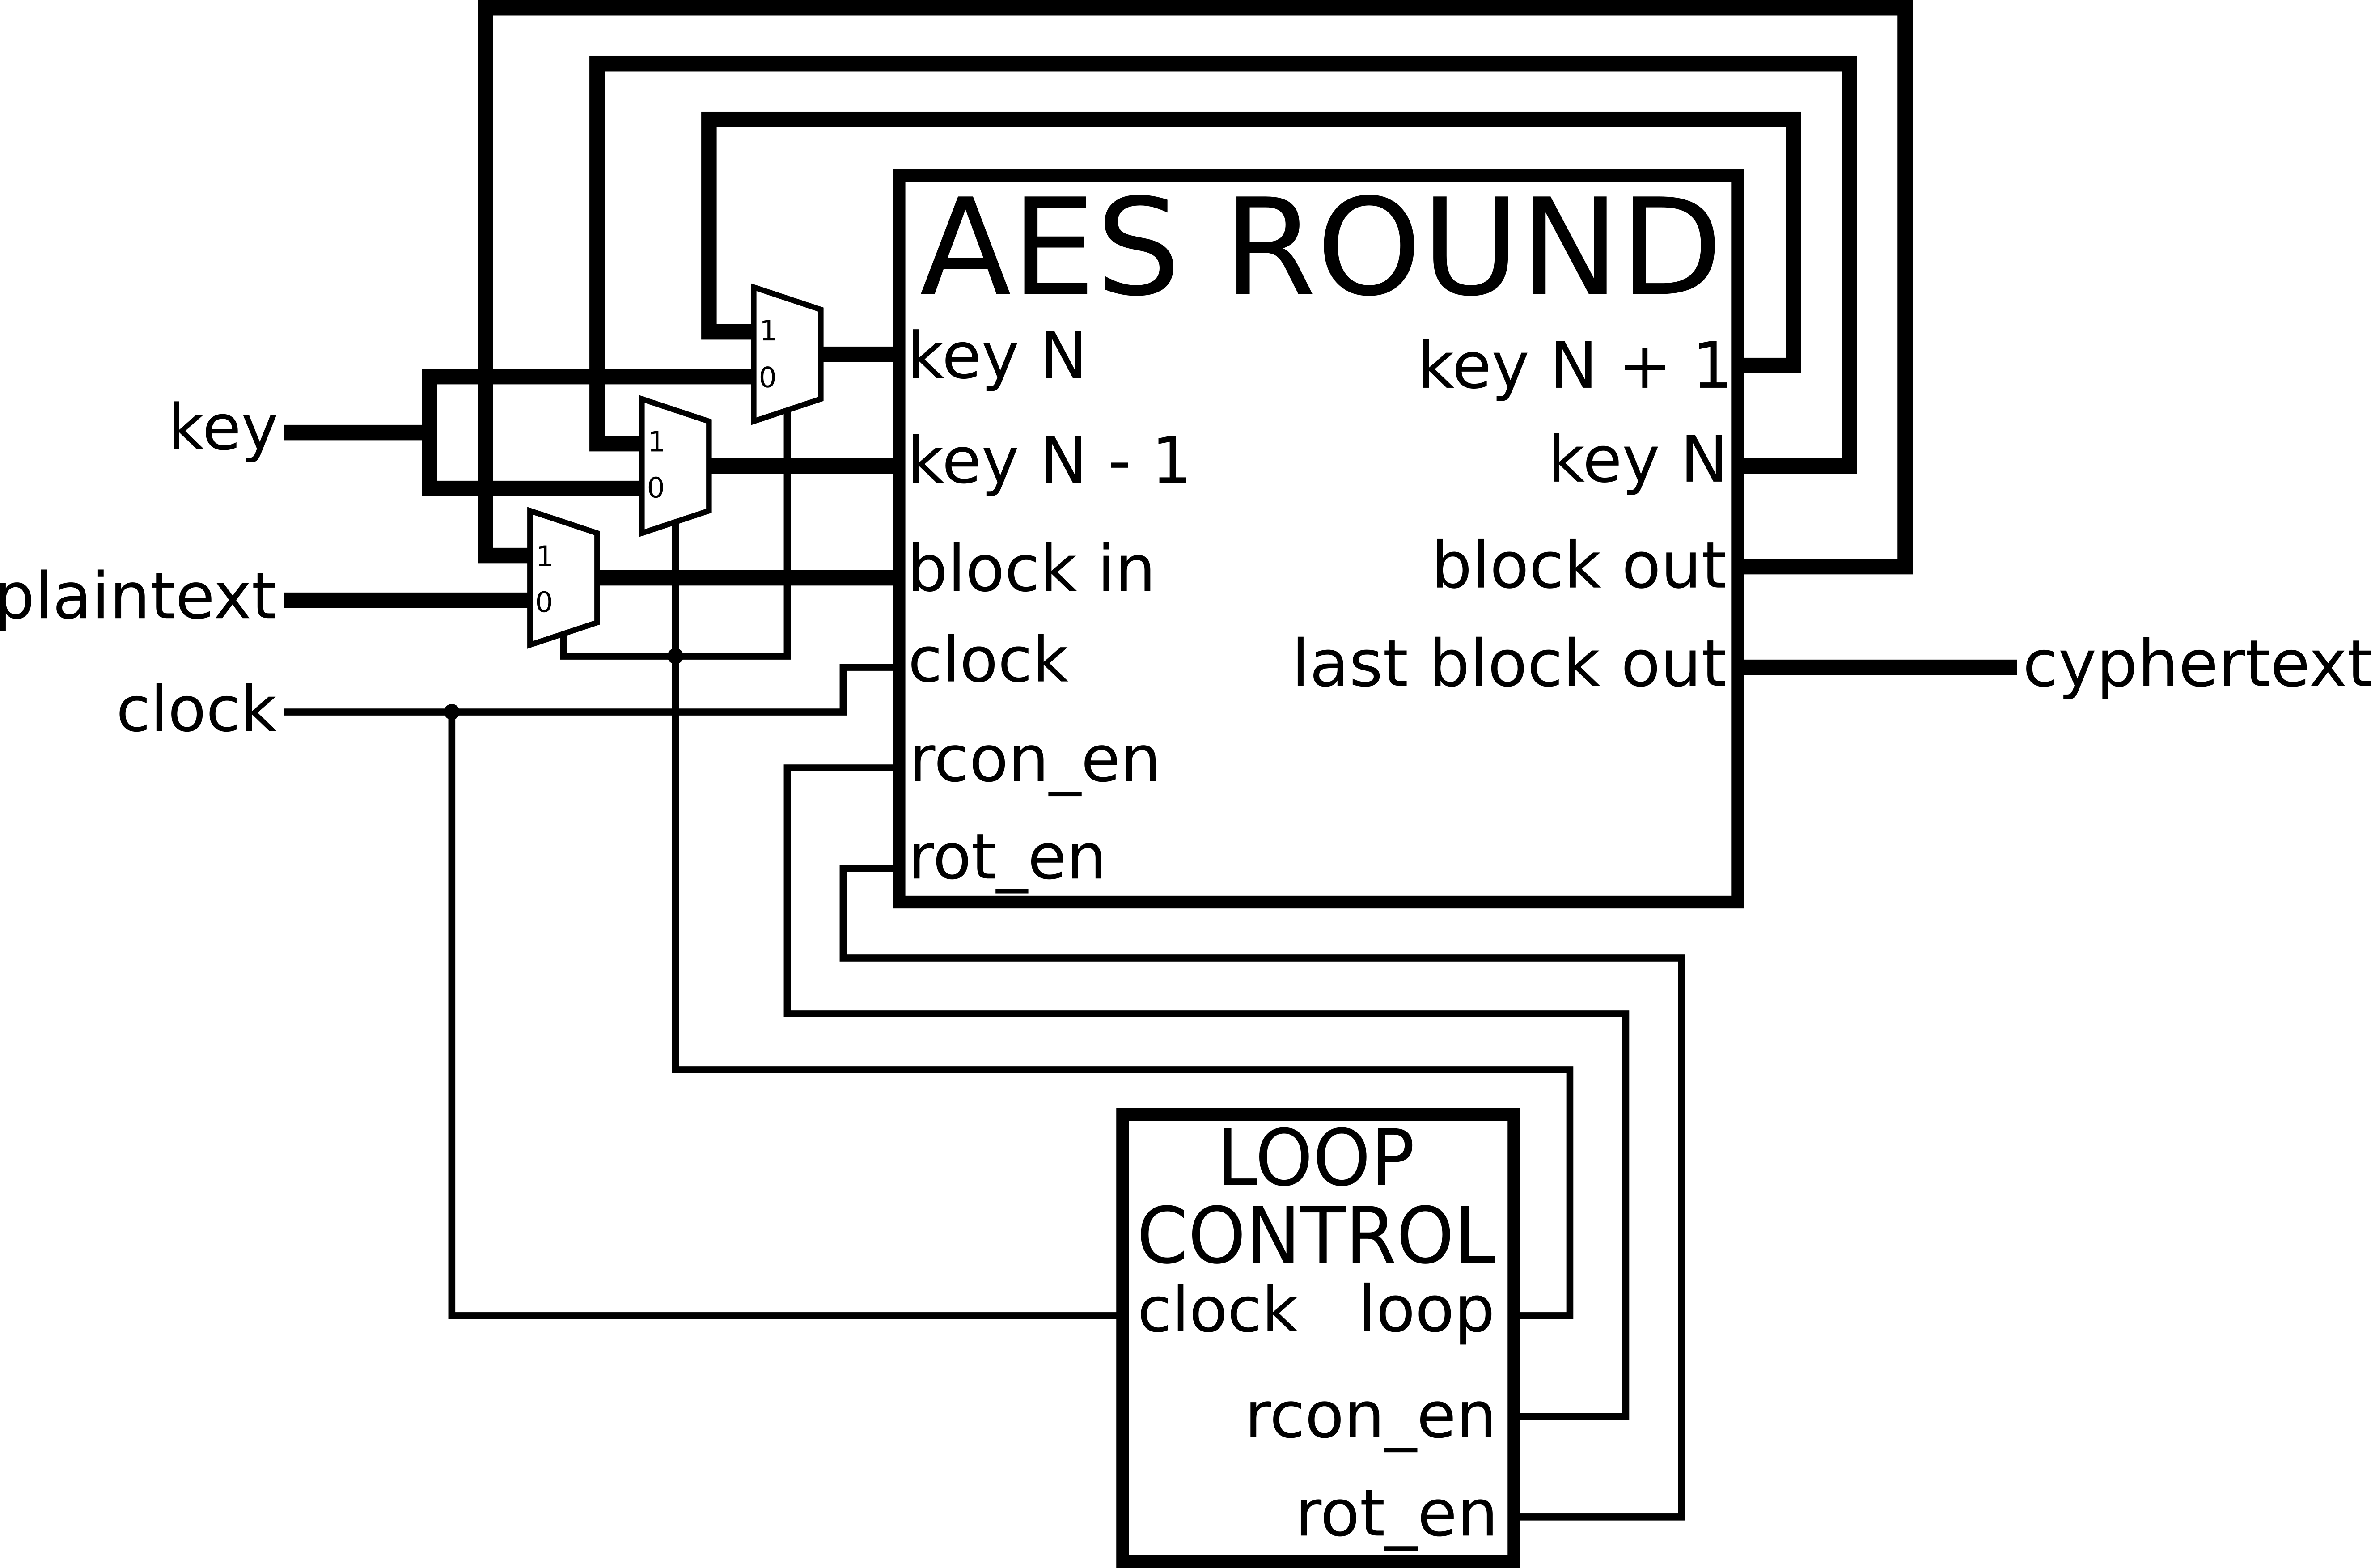
\includegraphics[scale=2]{rolled-loop}
\caption{Rolled up AES architecture}
\label{fig:rolled-loop}
\end{figure}

AES round design is based on \textit{Pipelined unrolled architecture with stages containing one ALM} to take advantage of pipelining and optimal round pipeline structure (stages containing one ALM). Each block of plaintext is processed by AES round 14 times. Iteration process is controlled by \textit{loop} signal, which indicates when encryption is done and new block should be input. 

AES rounds are not all the same - only in every other's round key expansion routine \textit{Rot} and \textit{Rcon} (fig. \ref{fig:aes-round-stages}) operations are performed. This requires addition of extra control logic to orchestrate execution of each loop iteration: \textit{rcon\_word} and \textit{rot\_en} signals. Their purpose is to enable corresponding operations every other round.

% Last AES round is different from previous ones in that it does not perform MixColumns transformation. To make it possible to reuse one round implementation for entire AES encryption process its original design was slightly altered (before fig. \ref{fig:high-speed-pipe-full}, after fig. \ref{fig:rolled-high-speed-pipe-full}). Before this modification, parallel to calculation of $N^{th}$ round was key expansion for $(N + 2)^{th}$ round. After modification, parallel to calculation of $N^{th}$ round is key expansion for $(N + \textbf{1})^{th}$ round. This modification is only a slight rearrangement of the pipeline which allows for more elegant design and does not change the complexity of the circuit. 

This design is capable of operating at \textbf{450MHz}, which is an improvement over \textit{Pipelined unrolled architecture with stages containing one ALM}. This is due to this circuit consuming less FPGA resources, which reduces logic congestion and allows for more efficient routing. As reported by compiler, this design uses \textbf{1423} FPGA ALMS (excluding 806 elements required for testing circuit). Encrypting a block of data requires \textbf{154} clock cycles.

\begin{figure}[!h]
\centering

\includegraphics[scale=3]{pipeline-flow}
\caption{Flow of data through pipelined AES round}
\label{fig:pipeline-flow}
\end{figure}

Although this circuit is rolled up, it is still capable of encrypting 11 different blocks of data concurrently. This is because AES round circuit remains pipelined. Flow of data through AES round can be observed in figure \ref{fig:pipeline-flow}. For the purpose of this research a version of this architecture in which all 11 blocks have to be provided in consecutive clock cycles was implemented. Using appropriate multiplexing it is possible to implement it as a circuit which can encrypt 11 independent streams of blocks, not necessarily provided in consecutive clock cycles. Author leaves it up to the Reader to modify his design accordingly.

Due to existence of pipeline in AES round, this architecture is capable of encrypting data with throughput of \textbf{4,1Gb/s}:
\begin{equation}
11 * 450MHz * 128b / 154 \approx 4,1Gb/s
\end{equation}


\subsubsection{Pipelined rolled up architecture using on-chip memory}

This architecture is based on \textit {Pipelined rolled up architecture with stages containing one ALM}. In this approach SubBytes transformation is implemented using on-chip memory, which stores an SBox -- look up table of substitution bytes. The circuit contains one such SBox, which is reused for all lookups (16 in SubButes transformation and 4 in key expansion routine).

This design is capable of operating at \textbf{315MHz}, which is the limit of on-chip memory for Altera Cyclone V Devices \cite[Table 27]{cycloneVDatasheet}. As reported by compiler, this design uses \textbf{725} FPGA ALMS (excluding 806 elements required for testing circuit) and \textbf{2048} memory bits. Circuit operates with throughput of \textbf{130,9Gb/s} and encrypting a block of data takes \textbf{308} clock cycles.

\newpage

\subsubsection{Results summary}

Achieved results and parameters of all tested architectures are summarized in table \ref{tab:table-summary}.

\begin{table}[!h]
\noindent\makebox[\textwidth]{%
\begin{tabular}{|c|c|c|c|c|c|}
	\hline 
	\multicolumn{1}{|c|}{\bfseries Architecture} & 
	\multicolumn{1}{c|}{\bfseries Max frequency} & 
	\multicolumn{1}{c|}{\bfseries Throughput} & 
	\multicolumn{1}{c|}{\bfseries Resource usage} & 
	\multicolumn{1}{c|}{\bfseries Clock cycles} & 
	\multicolumn{1}{c|}{\bfseries Latency} \\

	\hline 
	A \footnote{Simple asynchronous architecture} & 20M block per second & 2,5Gb/s & 20797 ALM & - & 50ns \\
	\hline 
	B \footnote{Pipelined unrolled architecture with stages of equal critical path length} & 362MHz & 46,3Gb/s & 12564 ALM & 84 & 232ns \\
	\hline 
	C \footnote{Pipelined unrolled architecture with stages containing one ALM} & 401MHz & 51,3Gb/s & 18078 ALM & 154 & 384ns \\
	\hline 
	D \footnote{Pipelined rolled up architecture with stages containing one ALM} & 450MHz & 4,1Gb/s & 1423 ALM & 154 & 342ns \\
	\hline 
	E \footnote{Pipelined rolled up architecture using on-chip memory} & 315MHz & 130,9Mb/s & 725 ALM + 2kb mem & 308 & 978ns \\
	\hline 
\end{tabular}
}
\caption{\label{tab:table-summary} Results summary}
\end{table}

Proposed AES encryption circuit designs have different performance characteristics:
\begin{itemize}

\item \textit{Simple asynchronous architecture} has the lowest latency because its encryption process occurs with the speed of signal propagation. It is not slowed down by delays introduced by flip-flops in pipelined architectures. It also does not suffer from uneven signal propagation time of pipeline stages. Low latency, however, comes at the cost of the highest FPGA resource usage and relatively low throughput.

\item \textit{Pipelined unrolled architecture with stages of equal critical path length} is moderate in all categories, among tested solutions its neither the most efficient nor does not consume the least amount of FPGA resources. With the highest throughput to resource usage ratio it is the most balanced design.

\item \textit{Pipelined unrolled architecture with stages containing one ALM} has the highest throughput at the cost of high resource usage.

\item \textit{Pipelined rolled up architecture with stages containing one ALM} in a looped version of \textit{Pipelined unrolled architecture with stages containing one ALM} which implements in hardware only 1 instance of AES encryption and creates a loop around it. With very similar throughput to resource usage ratio it provides a more flexibly scalable alternative to previous architecture.

\item \textit{Pipelined rolled up architecture using on-chip memory} uses the least amount of FPGA resources, but also has the lowest throughput out of the tested solutions. Unlike other designs it uses on-chip memory.

\end{itemize}
